%!TEX root=paper/paper.tex
\begin{figure}[H]
\centering
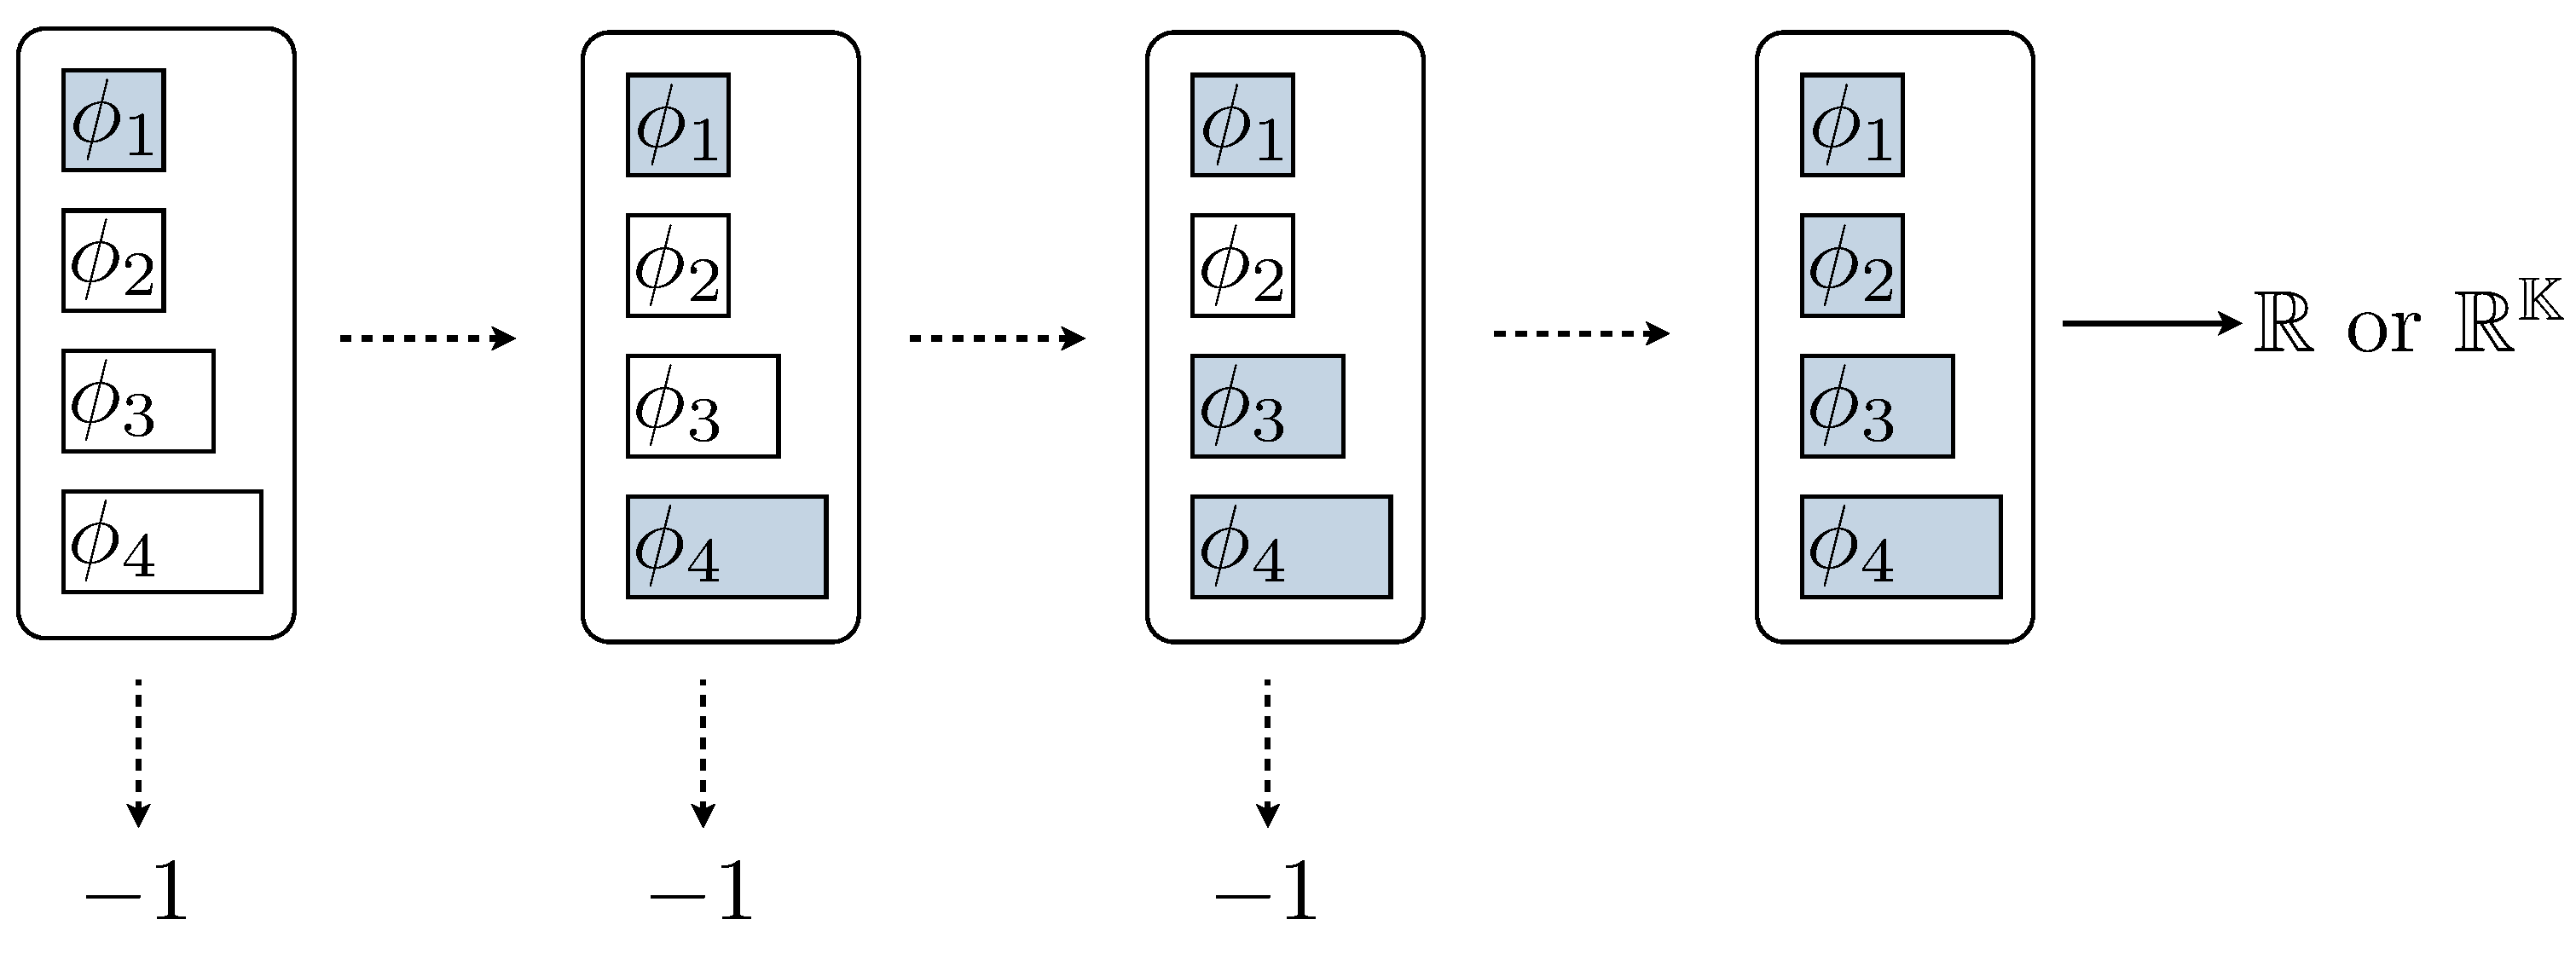
\includegraphics[width=.9\linewidth]{../../figures/models/cascade}
\caption[Sequential feature selection: cascade models]{
Sequential feature selection: \textbf{Cascade}.
In addition to the feature computation actions, the classifier is augmented with a rejection action.
The cascade is Anytime in a limited way, as only the rejection answer can be given before all features are evaluated.
The fixed order of the cascade is not robust to the fact that different images benefit from different features.
}\label{fig:model_cascade}
\end{figure}

\begin{figure}[H]
\centering
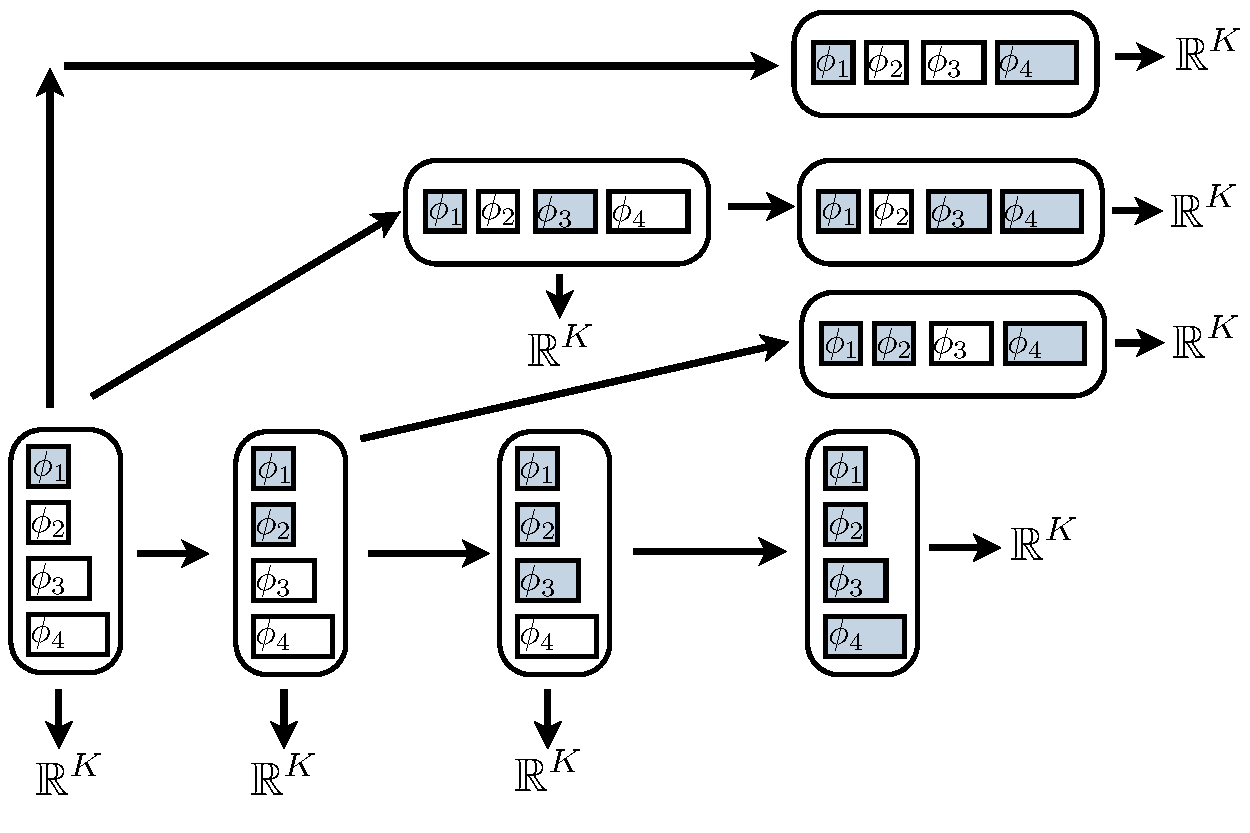
\includegraphics[width=.9\linewidth]{../../figures/models/benbouzid}
\caption[Sequential feature selection: Markov Decision DAG]{
The \textbf{MD-DAG} method \parencite{Benbouzid-ICML-2012} augments the traditional cascade with an additional Skip action, which allows learning a more robust policy.
}\label{fig:model_mddag}
\end{figure}

\begin{figure}[H]
\centering
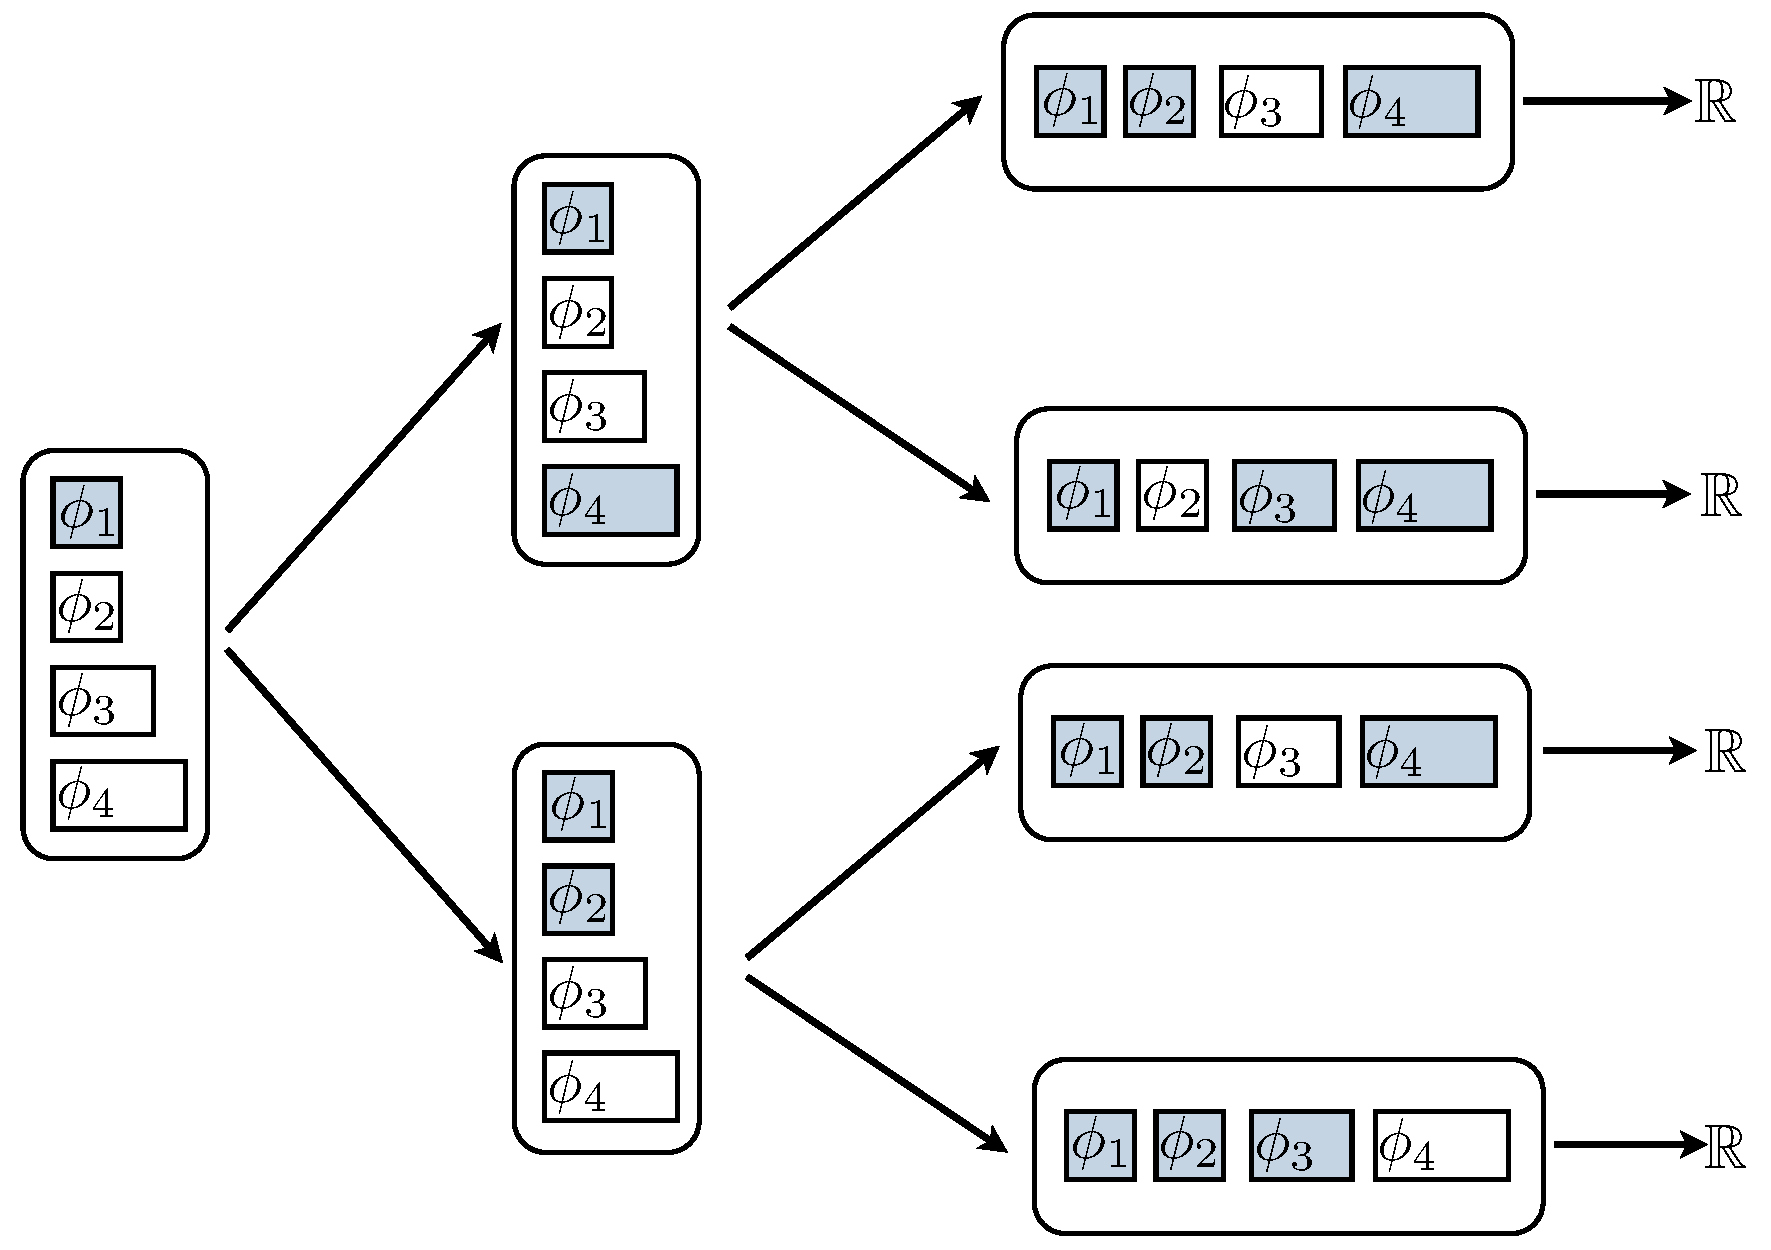
\includegraphics[width=.9\linewidth]{../../figures/models/tree}
\caption[Sequential feature selection: tree-based]{
\textbf{Tree-based} methods such as \cite{Xu-ICML-2012} find a tree-structured policy for computing features.
Classification answers are given only at the leaf nodes.
}\label{fig:model_tree}
\end{figure}

\begin{figure}[H]
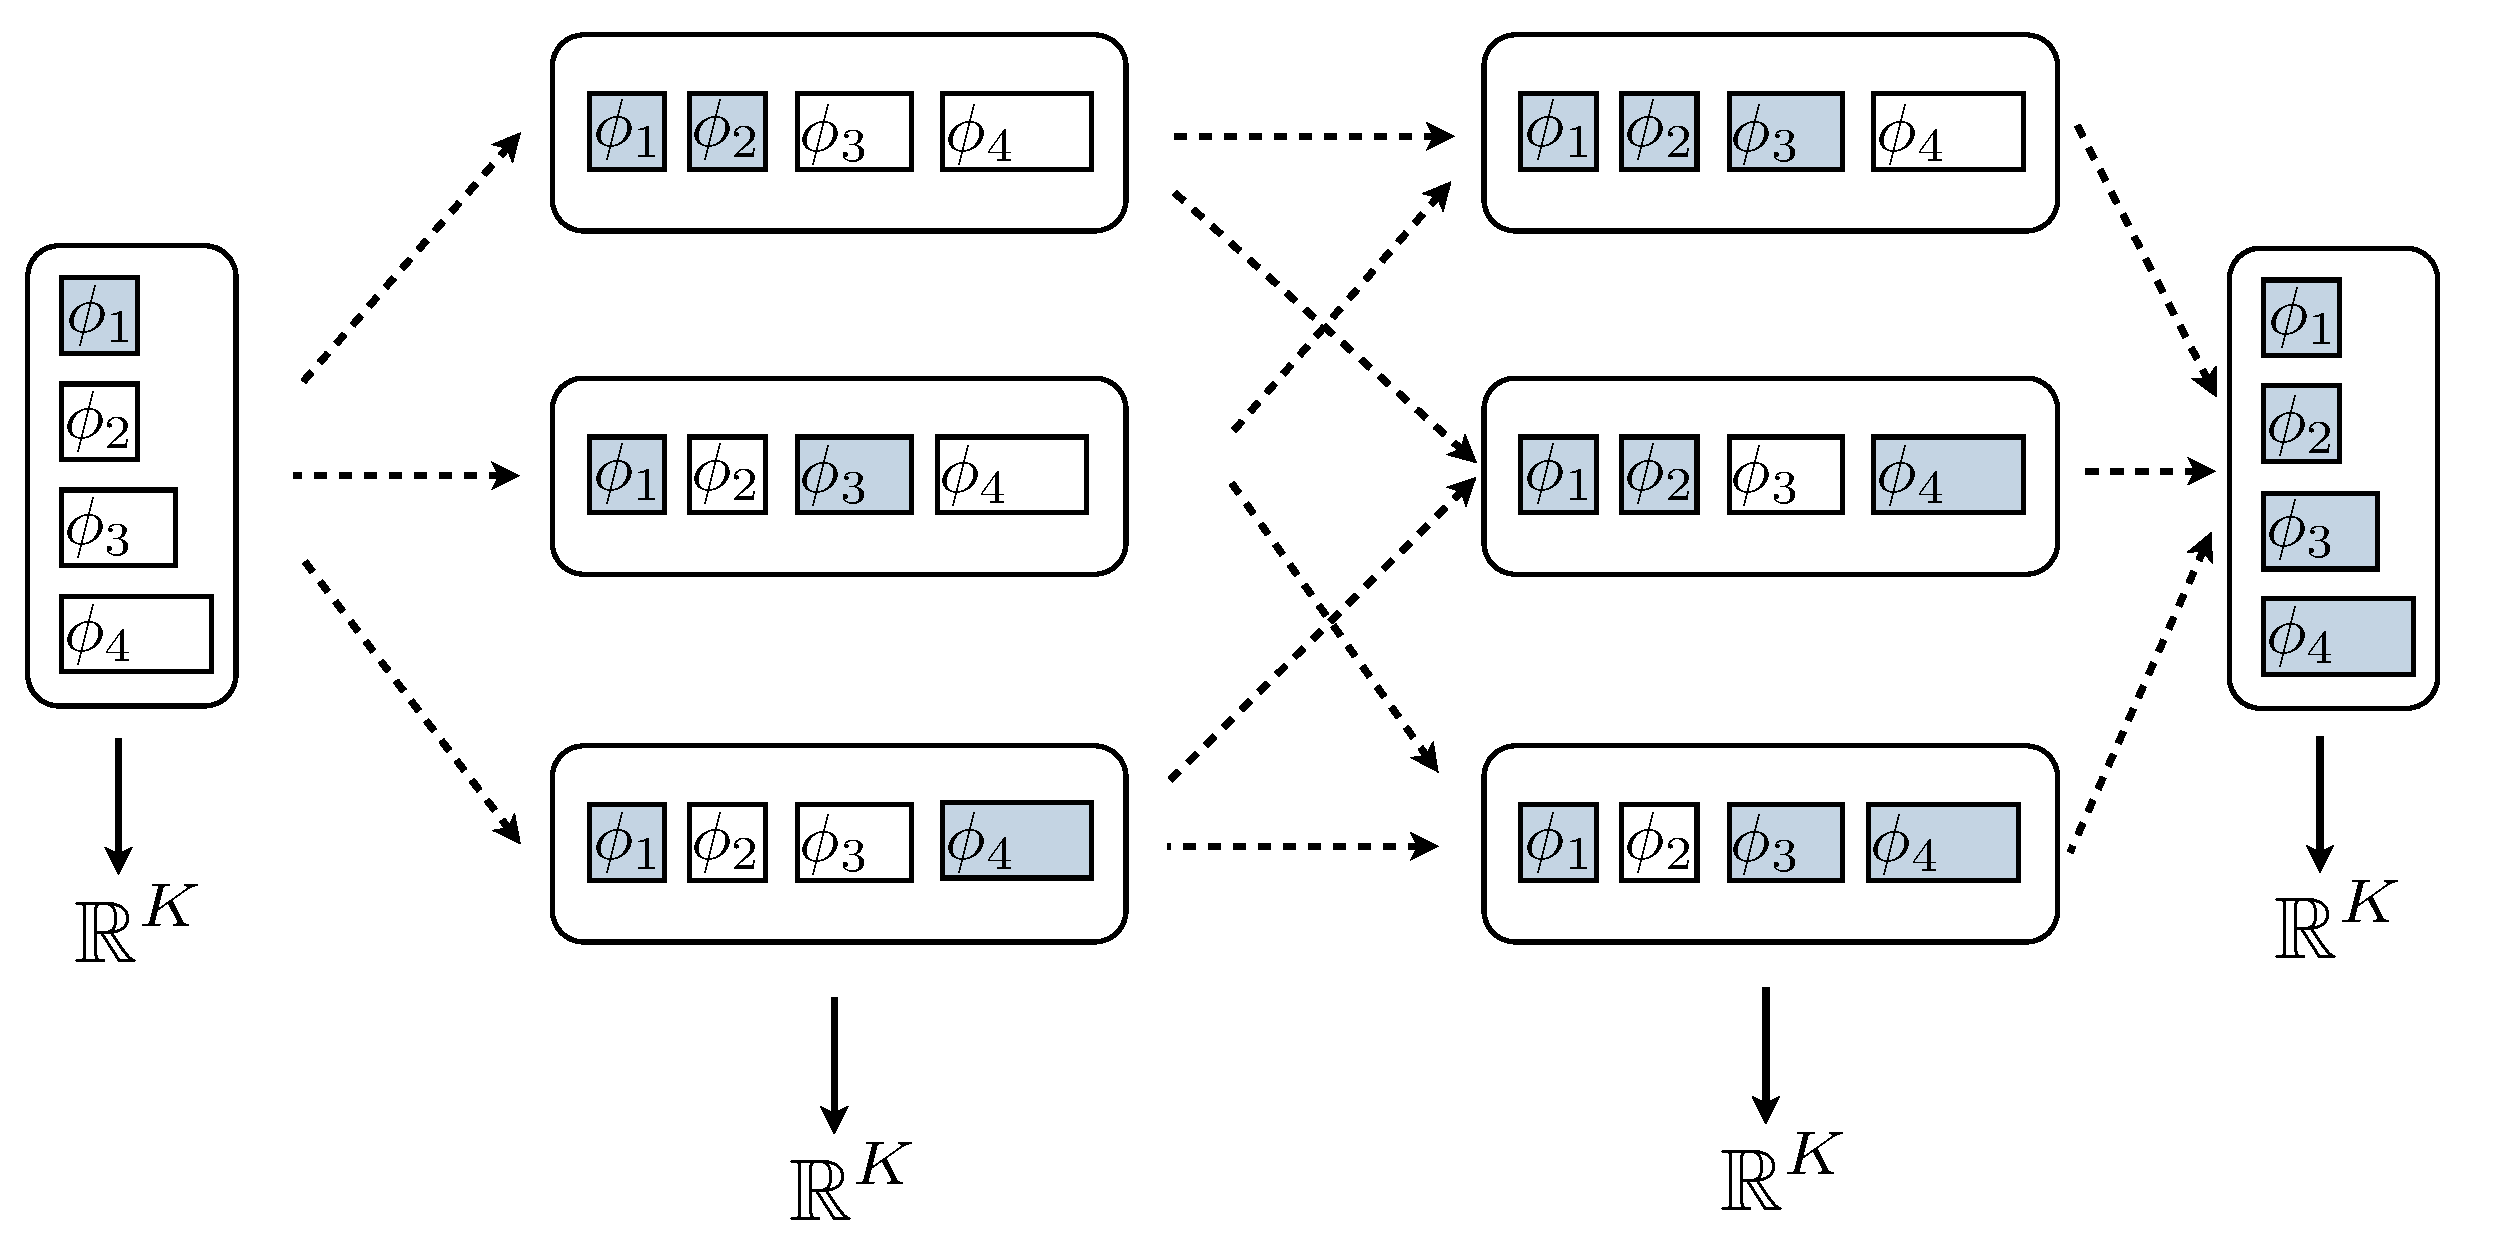
\includegraphics[width=\linewidth]{../../figures/models/dag}
\caption[Sequential feature selection: general DAG]{
In this work and in methods such as \cite{Gao-NIPS-2011}, the policy is a \textbf{general DAG} over selected-feature subsets, which allows actions to be taken in an entirely flexible order.
We are also able to give the classification answer from all states, making our work truly Anytime.
}\label{fig:model_dag}
\end{figure}
